\clearpage
\begin{explanationbox}
\textbf{从初中反比例函数出发：面积不变，究竟什么没变？}

初中学过 $Y=K/X$（$K\ne0$）：设点 $M=(X,Y)$，
以坐标轴为边作矩形，其面积为
\[
\boxed{S_{\text{矩形}}=|X|\,|Y|=|K|}.
\]
\textbf{关键不是 $X$、$Y$ 分别不变，而是它们的乘积 $XY$ 不变。}
矩形的两个邻边沿着互相垂直的坐标轴；若换成\emph{两条倾斜的固定方向}，
对应的就是斜向平行四边形，面积仍由两条边的“位移系数乘积”控制。

\textbf{把本题改写成一个熟悉的反比例函数：}
令 $k=b/a$，以两渐近线方向分解 $P$：
\[
Q=(u,ku),\quad R=(v,-kv),\quad P=Q+R.
\]
于是 $x=u+v$、$y=k(u-v)$，从而
\[
\boxed{(u+v)^2-(u-v)^2=4uv=a^2}
\quad\Longleftrightarrow\quad
\boxed{v=\frac{a^2}{4u}}.
\]
\textbf{认知桥梁：}初中是 $XY=K$ 对应矩形面积恒定；
这里是 $uv=a^2/4$ 对应倾斜平行四边形面积恒定。
不要把坐标系中的 $x,y$ 误认成斜向坐标 $u,v$，
也不要把倾斜平行四边形直接当矩形：还需说明\emph{面积系数}为何是 $2k$。

\textbf{从几何上读出 $2k$：}
作竖直剪切 $(X,Y)\mapsto(X,Y-kX)$。
它只是把每条竖直截线整体上下平移，不改变面积。
剪切后 $O=(0,0)$、$Q=(u,0)$、$R=(v,-2kv)$，
原平行四边形变为底长 $|u|$、高 $2k|v|$ 的平行四边形，故
\[
S=|u|\cdot2k|v|=2k|uv|
=2\cdot\frac ba\cdot\frac{a^2}{4}
=\boxed{\frac{ab}{2}}.
\]
\textbf{识别主线：}\emph{旧知识（反比例函数）}
$\to$ \emph{换两条斜轴} $\to$ \emph{平方差变乘积}
$\to$ \emph{平行四边形面积不变}。
\end{explanationbox}

\clearpage
\begin{explanationbox}
\textbf{几何直觉一：双曲线就是“两个平方的差固定”。}

\begin{center}
% Exact model a=3,b=2,u=9/4,v=1; component arrows are directed.
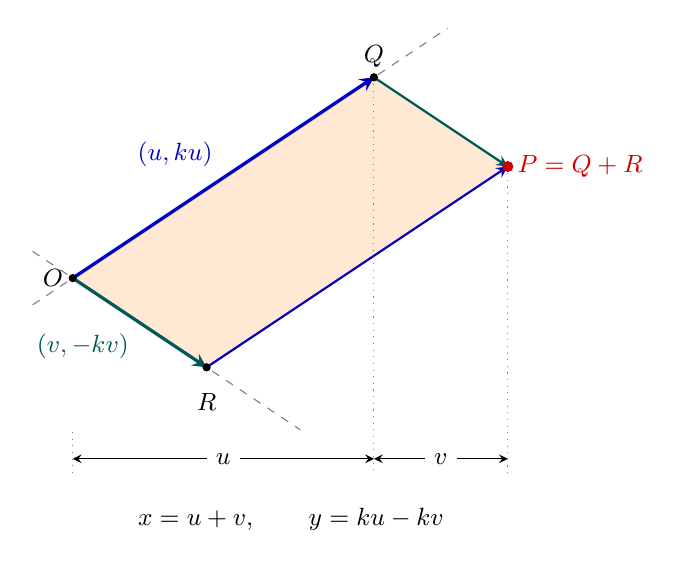
\begin{tikzpicture}[x=1.7cm,y=1.7cm,>=stealth,font=\small]
\coordinate (O) at (0,0); \coordinate (Q) at (2.25,1.5);
\coordinate (R) at (1,-2/3); \coordinate (P) at (3.25,5/6);
\fill[orange!17] (O)--(Q)--(P)--(R)--cycle;
\draw[gray,dashed] (-.3,-.2)--(2.8,28/15);
\draw[gray,dashed] (-.3,.2)--(1.7,-17/15);
\draw[->,blue!75!black,very thick] (O)--(Q) node[midway,above left] {$(u,ku)$};
\draw[->,teal!70!black,very thick] (O)--(R) node[midway,below left] {$(v,-kv)$};
\draw[->,teal!70!black,thick] (Q)--(P);
\draw[->,blue!75!black,thick] (R)--(P);
\draw[gray,dotted] (0,-1.15)--(0,-1.45) (Q)--(2.25,-1.45) (P)--(3.25,-1.45);
\draw[<->] (0,-1.35)--(2.25,-1.35) node[midway,fill=white] {$u$};
\draw[<->] (2.25,-1.35)--(3.25,-1.35) node[midway,fill=white] {$v$};
\node at (1.63,-1.8) {$x=u+v,\qquad y=ku-kv$};
\fill (O) circle(1.5pt) node[left] {$O$};
\fill (Q) circle(1.5pt) node[above] {$Q$};
\fill (R) circle(1.5pt) node[below=6pt] {$R$};
\fill[red!80!black] (P) circle(2pt) node[right] {$P=Q+R$};
\end{tikzpicture}

\end{center}

图中记 $k=b/a>0$，两条有向边首尾平移后得到 $P=Q+R$。
横向分量相加、纵向分量相减，直接读出 $x=u+v$、$y=k(u-v)$。
因此不用解交点，只需平方差恒等式：
\[
\underbrace{x^2-\frac{y^2}{k^2}}_{\text{双曲线要求 }=a^2}
=(u+v)^2-(u-v)^2=\boxed{4uv}.
\]
而这个平行四边形的面积恰为 $2k|uv|$，因此
\[
S=2k|uv|=\frac{k}{2}\,\underbrace{|4uv|}_{=a^2}
=\boxed{\frac{ka^2}{2}=\frac{ab}{2}}.
\]
\textbf{与初中的对应关系：}$uv=a^2/4$ 就是 $v=(a^2/4)/u$；
因此本结论可以看作\textbf{反比例函数定面积性质在斜向坐标中的升级}。

\textbf{最低记忆负担：}把坐标看成“沿两条渐近线走了多少”；
\textbf{差平方 $\to$ 乘积 $4uv$ $\to$ 面积}。点动时 $u,v$ 可变，
但 $uv=a^2/4$ \textbf{不变}。
\end{explanationbox}

\clearpage
\begin{explanationbox}
\textbf{几何直觉二：为什么需要除以 $\sin\theta$？}

\begin{center}
% a=3,b=2; u=9/4,v=1. Orthogonal feet are computed exactly.
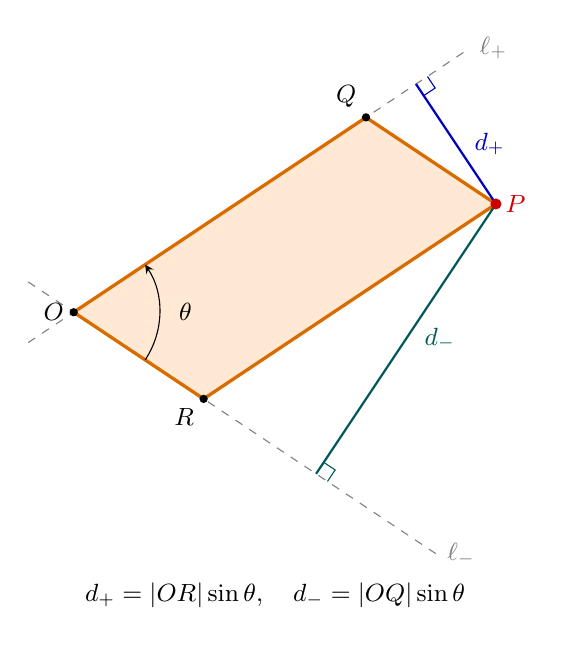
\begin{tikzpicture}[x=1.65cm,y=1.65cm,>=stealth,font=\small]
\coordinate (O) at (0,0); \coordinate (Q) at (2.25,1.5);
\coordinate (R) at (1,-2/3); \coordinate (P) at (3.25,5/6);
\coordinate (A) at (137/52,137/78);
\coordinate (B) at (97/52,-97/78);
\fill[orange!17] (O)--(Q)--(P)--(R)--cycle;
\draw[gray,dashed] (-.35,-7/30)--(3.05,61/30) node[right] {$\ell_+$};
\draw[gray,dashed] (-.35,7/30)--(2.8,-28/15) node[right] {$\ell_-$};
\draw[orange!85!black,very thick] (O)--(Q)--(P)--(R)--cycle;
\draw[blue!75!black,thick] (P)--(A) node[midway,right=3pt] {$d_+$};
\draw[teal!70!black,thick] (P)--(B) node[midway,right=3pt] {$d_-$};
% right angle markers at A and B
\draw[blue!75!black] (2.7231,1.8141)--(2.7819,1.7259)--(2.6937,1.6671);
\draw[teal!70!black] (1.9536,-1.3024)--(2.0124,-1.2142)--(1.9242,-1.1554);
\draw[->] (0.55,-.3667) arc[start angle=-33.6901,end angle=33.6901,radius=.661];
\node at (.86,0) {$\theta$};
\fill (O) circle(1.5pt) node[left] {$O$};
\fill (Q) circle(1.5pt) node[above left] {$Q$};
\fill (R) circle(1.5pt) node[below left] {$R$};
\fill[red!80!black] (P) circle(2pt) node[right] {$P$};
\node at (1.55,-2.18) {$d_+=|OR|\sin\theta,\quad d_-=|OQ|\sin\theta$};
\end{tikzpicture}

\end{center}

图中两条垂线给出两组平行线之间的距离 $d_+$、$d_-$，
夹角 $\theta\in(0,\pi)$。把图下注明的边长与垂距关系
代入 $S=|OQ|\,|OR|\sin\theta$，得到
\[
\boxed{S=\frac{d_+d_-}{\sin\theta}}.
\]
这就是通用的\textbf{“两组平行线围面积”公式}。
\textbf{注意：}不是 $d_+d_-$；两条边不垂直时，必须考虑夹角。

本题中 $d_+d_-$ 含有
$|bx-ay|\,|bx+ay|=|b^2x^2-a^2y^2|$；
双曲线正好把这个\textbf{乘积}固定为 $a^2b^2$。
因此面积不随 $P$ 改变，并非单独的某条边长或某个距离固定。

\textbf{几何直觉三：左右支无需分开。}
当 $P$ 移到左支时，沿两条渐近线的有向坐标 $u,v$ 同时变负，
但 $uv>0$、面积取绝对值不变；同理，$y$ 的正负也不影响 $S$。
\end{explanationbox}


\clearpage
\begin{explanationbox}
\textbf{为什么面积定值还能控制周长？}

两条渐近线方向向量可取 $(a,b)$ 与 $(a,-b)$，
邻边长度分别为
\[
|OQ|=|u|\sqrt{1+k^2},\qquad |OR|=|v|\sqrt{1+k^2}.
\]
由于 $uv=a^2/4$、$k=b/a$，
\[
\boxed{|OQ|\cdot|OR|=(1+k^2)|uv|=\frac{a^2+b^2}{4}
=\frac{c^2}{4}},\quad c^2=a^2+b^2.
\]
所以邻边长度虽然分别变化，\textbf{乘积不变}；
再由 $A+B\ge2\sqrt{AB}$ 得四边形周长
\[
L=2\bigl(|OQ|+|OR|\bigr)\ge2c.
\]
当且仅当 $|OQ|=|OR|$，即 $u=v$、$y=0$、
$P=(\pm a,0)$ 时取等号。这也解释了\textbf{为什么顶点恰好对应菱形、周长最小}。

\textbf{固定焦距参数的进一步思考：}
若 $c$ 固定，$a^2+b^2=c^2$，则 $2ab\le a^2+b^2$，因此
\[
0<S=\frac{ab}{2}\le\boxed{\frac{c^2}{4}}.
\]
上界在 $a=b=c/\sqrt2$ 时达到；因 $a,b>0$，下界 $0$\textbf{不能取到}。
\end{explanationbox}
